
Let $X$ and $Y$ be two independent random variables. \\
Let $Z$ be another random variable where $Z=X+Y$
$X \in \sbrak{0,10}$,$Y \in \sbrak{0,20}$,$Z \in \sbrak{0,30}$
\begin{align}
\int_{0}^{10} p_X(x) \mathrm{dx} &=1  \\
\therefore p_X(x)&=\frac{1}{10} \label{me2019-28:px}
\end{align}
The PDF for $X$ is
\begin{align}
p_X(x)  = 
\begin{cases}
     \frac{1}{10} & 0 \leq x \leq 10\\
     0 & otherwise \label{me2019-28:1}
\end{cases}
\end{align}
Similarly,PDF for $Y$ is
\begin{align}
p_{Y}(y)  = 
\begin{cases}
     \frac{1}{20} & 0 \leq y \leq 20 \\
      0 & otherwise \label{me2019-28:2}
\end{cases}
\end{align}
$x=z-y$.Using this pdf of X can be written as
\begin{align}
p_X(z-y)  = 
\begin{cases}
    \frac{1}{10} & 0 \leq z-y \leq 10\\
    0 & otherwise \label{me2019-28:3}
\end{cases}
\end{align}
\begin{align}
   z-10 &\leq y \leq z \label{me2019-28:4} \\
   0 &\leq y \leq 20 \label{me2019-28:5}
\end{align}
pdf of $Z$ by convolution can be written as
\begin{align}
 p_Z(z) =  \int_{- \infty}^{\infty} p_X(z-y)p_Y(y) \mathrm{dy} \label{me2019-28:pz}
\end{align}
From \ref{me2019-28:2} and \ref{me2019-28:3}
\begin{align}
 p_Z(z) = \frac{1}{200} \int_{- \infty}^{\infty} \mathrm{dy} \label{me2019-28:6}
\end{align}
For $0 \leq z \leq 10$  
\begin{align}
p_Z(z) &= \frac{1}{200}  \int_{0}^{z}\mathrm{dy}  \\
       &= \frac{z}{200} \label{me2019-28:7}
\end{align}
For $ 10 < z \leq 20 $,
\begin{align}
p_Z(z) &= \frac{1}{200}  \int_{z-10}^{z}\mathrm{dy}  \\
        &= \frac{1}{20} \label{me2019-28:8}
\end{align}
For $ 20 < z \leq 30 $,
\begin{align}
p_Z(z) &=\frac{1}{200}  \int_{z-10}^{20}\mathrm{dy}  \\
       &= \frac{30-z}{200} \label{me2019-28:9}
\end{align}
$\therefore$ PDF of $Z$ is as follows
\begin{align}
p_{Z}(z)  = 
\begin{cases}
  \frac{z}{200}& 0 \leq z \leq 10 \\
  \frac{1}{20} & 10 < z \leq 20 \\
  \frac{30-z}{200} & 20 < z \leq 30 \\
  0 & otherwise \label{me2019-28:10}
\end{cases}
\end{align}
\begin{equation}
F_Z(z) = \Pr(Z \leq z) \label{me2019-28:cdf}
\end{equation}
The CDF  of $Z$ is as follows:
\begin{align}
F_Z(z)  = 
\begin{cases}
  0 & z < 0 \\
  \frac{z^2}{400} & 0 \leq z \leq 10 \\
  \frac{z-5}{20} & 10< z \leq 20 \\
  \frac{60z -500 -z^2}{400} & 20< z \leq 30 \\
  1 & z > 30 \label{me2019-28:11}
\end{cases}
\end{align}
\begin{align}
\Pr(z > 20)&= 1- F_Z(20) \\
           &=\frac{1}{4} \label{me2019-28:12} \\
\therefore \Pr(x+y>20)&=\frac{1}{4}=0.25
\end{align}
\begin{figure}[htb!]
\begin{center}
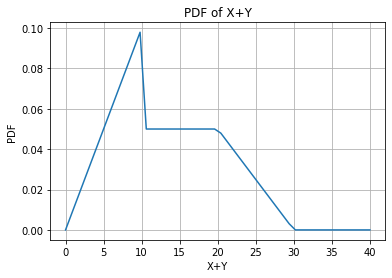
\includegraphics[width=0.5\textwidth]{solutions/me/2019/28/figures/assignment6pdf.png}
\end{center}
\end{figure}

\begin{figure}[htb!]
\begin{center}
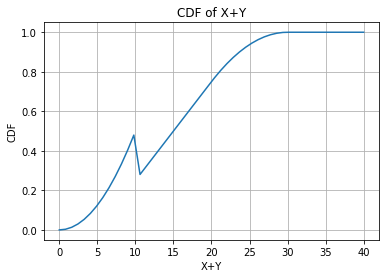
\includegraphics[width=0.5\textwidth]{solutions/me/2019/28/figures/assignment6cdf.png}
\end{center}
\end{figure}

